\documentclass[12pt,letterpaper,fleqn]{article}
\usepackage[utf8]{inputenc}	
\usepackage{amsmath,amsthm,amsfonts,amssymb,amscd}
\usepackage{multirow,booktabs}
\usepackage[table]{xcolor}
\usepackage{amssymb}
\usepackage{fullpage}
\usepackage{lastpage}
\usepackage{enumitem}
\usepackage{fancyhdr}
\usepackage{mathrsfs}
\usepackage{wrapfig}
\usepackage{graphicx}
\graphicspath{ {./img/} }
\usepackage{setspace}
\usepackage{calc}
\usepackage{multicol}
\usepackage{cancel}
\usepackage[margin=3cm]{geometry}
\usepackage{floatrow}
\newlength{\tabcont}
\addtolength{\jot}{10pt}
\setlength{\parindent}{0.0in}
\setlength{\parskip}{0.05in}
\title{Assignment 0 - Vivek T, 17397}
\newcommand\course{17397}	
\newcommand\semester{2021} 
\newcommand\yourname{Vivek T}  
\theoremstyle{definition}
\usepackage{mathtools}
\DeclarePairedDelimiterX\set[1]\lbrace\rbrace{\def\given{\;\delimsize\vert\;}#1}
\newtheorem{defn}{Definición}
\newtheorem{reg}{Regla}
\newtheorem{ejer}{EJERCICIO}
\pagestyle{fancyplain}
\headheight 32pt
\lhead{\yourname\ \vspace{0.1cm} \\ \course}
\chead{\textbf{\Large DS284 Assignment-0}}
\rhead{16/08/2021}
\begin{document}
\textbf{(1.a)} Given:

\begin{equation}
\mathbb{V} = 
\set[\Bigg]{
\begin{pmatrix}
w\\
x\\
y\\
z\\
\end{pmatrix}
\given w - x - y + z = 0; w,x,y,z \in \mathbb{R}}
\end{equation}

Consider three vectors $u_1$, $u_2$ and $u_3$ such that $u_1, u_2, u_3 \in \mathbb{V}$.\\
Let 
\begin{equation*}
u_1 =
\begin{pmatrix}
w_1\\
x_1\\
y_1\\
z_1
\end{pmatrix}\texttt{,}~
u_2 = 
\begin{pmatrix}
w_2\\
x_2\\
y_2\\
z_2
\end{pmatrix}~\texttt{and}~
u_3 = 
\begin{pmatrix}
w_3\\
x_3\\
y_3\\
z_3
\end{pmatrix}
\end{equation*}
Checking for the conditions necessary for satisfying a real vector space,
\begin{enumerate}
\item Closure under addition property:
\begin{equation*}
\begin{split}
&u_1 + u_2 = 
\begin{pmatrix}
w_1 + w_2\\
x_1 + x_2\\
y_1 + y_2\\
z_1 + z_2
\end{pmatrix}\\
&(w_1 + w_2) -(x_1 + x_2) - (y_1 + y_2) + (z_1 + z_2)\\
&= (w_1 - x_1 - y_1 + z_1) + (w_2 - x_2 - y_2 + z_2)
\end{split}
\end{equation*}
Since $u_1,~u_2 \in \mathbb{V}$, $(w_1 - x_1 - y_1 + z_1) = 0 ~\texttt{and}~(w_2 - x_2 - y_2 + z_2) = 0$.
\begin{equation*}
\begin{split}
&\implies (w_1 - x_1 - y_1 + z_1) + (w_2 - x_2 - y_2 + z_2) = 0\\
&\implies u_1 + u_2 \in \mathbb{V}
\end{split}
\end{equation*}
Thus the closure under addition property is satisfied.\\

\item Commutative property
\begin{equation*}
\begin{split}
u_1 + u_2 &= 
\begin{pmatrix}
w_1 + w_2\\
x_1 + x_2\\
y_1 + y_2\\
z_1 + z_2
\end{pmatrix}\\
&= \begin{pmatrix}
w_2 + w_1\\
x_2 + x_1\\
y_2 + y_1\\
z_2 + z_1
\end{pmatrix} ~\because~ w,x,y,z \in \mathbb{R} \texttt{ obeys commutativity}\\
&= \begin{pmatrix}
w_2\\
x_2\\
y_2\\
z_2 
\end{pmatrix} + 
\begin{pmatrix}
w_1\\
x_1\\
y_1\\
z_1 
\end{pmatrix}\\
&= u_2 + u_1
\end{split}
\end{equation*}
Hence commutativity is satisfied.

\item Associative property
\begin{equation*}
\begin{split}
u_1 + (u_2 + u_3) &=
\begin{pmatrix}
w_1\\
x_1\\
y_1\\
z_1
\end{pmatrix} +
\begin{pmatrix}
w_2 + w_3\\
x_2 + x_3\\
y_2 + y_3\\
z_2 + z_3
\end{pmatrix}\\
&= \begin{pmatrix}
w_1 + w_2 + w_3\\
x_1 + x_2 + x_3\\
y_1 + y_2 + y_3\\
z_1 + z_2 + z_3
\end{pmatrix}\\
&= \begin{pmatrix}
w_1 + w_2\\
x_1 + x_2\\
y_1 + y_2\\
z_1 + z_2
\end{pmatrix} + 
\begin{pmatrix}
w_3\\
x_3\\
y_3\\
z_3
\end{pmatrix}\\
&= (u_1 + u_2) + u_3
\end{split}
\end{equation*}
Hence associativity is satisfied.

\item Zero vector
\begin{equation*}
\begin{split}
u_1 + 0 &= \begin{pmatrix}
w_1\\
x_1\\
y_1\\
z_1
\end{pmatrix} + 
\begin{pmatrix}
0\\
0\\
0\\
0
\end{pmatrix}\\
&= \begin{pmatrix}
w_1 + 0\\
x_1 + 0\\
y_1 + 0\\
z+1 + 0
\end{pmatrix}\\
&= \begin{pmatrix}
w_1\\
x_1\\
y_1\\
z_1
\end{pmatrix}, \because w,x,y,z \in \mathbb{R} \texttt{ obeys additive property}\\
&= u_1
\end{split}
\end{equation*}
Hence additivity property is satisfied for any $u_1 \in \mathbb{V}$

\item Additive inverse
$u_1 \in \mathbb{V}$.\\
 Then $ -1 \cdot u_1 \in \mathbb{V}$,\\
  since $ w_1 - x_1 - y_1 + z_1 = 0 \implies -1 \cdot w_1 + 1 \cdot x_1 + 1 \cdot y_1 - 1 \cdot z_1 = 0$\\
   and $ -w_1, -x_1, -y_1, -z_1 \in \mathbb{R}$.\\
   $\implies \forall u_1 \in \mathbb{V}, \exists -u_1 \in \mathbb{V}$ such that $ u_1  + (-u_1) = 0$, where $-u_1$ is the additive inverse.

\item Closure under scalar Multiplication
Let $c \in \mathbb{R}$.\\
Then,
\begin{equation*}
\begin{split}
c \cdot u_1 &= c \cdot \begin{pmatrix}
w_1\\
x_1\\
y_1\\
z_1
\end{pmatrix}\\
&= \begin{pmatrix}
c \cdot w_1\\
c \cdot x_1\\
c \cdot y_1\\
c \cdot z_1
\end{pmatrix}\\
\end{split}
\end{equation*}
$\because u_1 \in \mathbb{V}$, $w_1 - x_1 - y_1 + z_1 = 0$.\\
Multiplying both LHS and RHS by scalar constant $c$,\\
$ c \cdot (w_1 - x_1 - y_1 + z_1) = 0$.\\
$ \implies c \cdot w_1 - c \cdot x_1 - c \cdot y_1 + c \cdot z_1 = 0$\\
$ \implies c \cdot u_1 \in \mathbb{V}$.

\item Distributive property for scalar addition\\
Let $c,d \in \mathbb{R}$.\\
Then,
\begin{equation*}
\begin{split}
(c + d)\cdot u_1 &= (c + d) \cdot \begin{pmatrix}
w_1\\
x_1\\
y_1\\
z_1
\end{pmatrix}\\
&= \begin{pmatrix}
(c + d)\cdot w_1\\
(c + d)\cdot x_1\\
(c + d)\cdot y_1\\
(c + d)\cdot z_1
\end{pmatrix}\\
&= \begin{pmatrix}
c \cdot w_1 + d \cdot w_1\\
c \cdot x_1 + d \cdot x_1\\
c \cdot y_1 + d \cdot y_1\\
c \cdot z_1 + d \cdot z_1
\end{pmatrix}\\
&= \begin{pmatrix}
c \cdot w_1\\
c \cdot x_1\\
c \cdot y_1\\
c \cdot z_1
\end{pmatrix} +
\begin{pmatrix}
d \cdot w_1\\
d \cdot x_1\\
d \cdot y_1\\
d \cdot z_1
\end{pmatrix}\\
&= c \cdot \begin{pmatrix}
w_1\\
x_1\\
y_1\\
z_1
\end{pmatrix} +
d \cdot \begin{pmatrix}
w_1\\
x_1\\
y_1\\
z_1
\end{pmatrix}\\
&= c \cdot u_1 + d \cdot u_1
\end{split}
\end{equation*}
\newpage
\item Distribute property for vector addition
Let $c \in \mathbb{R}$.\\
Then,
\begin{equation*}
\begin{split}
c (u_1 + u_2) &= c \cdot \left(\begin{pmatrix}
w_1\\
x_1\\
y_1\\
z_1
\end{pmatrix} + 
\begin{pmatrix}
w_2\\
x_2\\
y_2\\
z_2
\end{pmatrix}\right)\\
&= c \cdot \begin{pmatrix}
w_1 + w_2\\
x_1 + x_2\\
y_1 + y_2\\
z_1 + z_2
\end{pmatrix} \\
&= \begin{pmatrix}
c \cdot (w_1 + w_2)\\
c \cdot (x_1 + x_2)\\
c \cdot (y_1 + y_2)\\
c \cdot (z_1 + z_2)
\end{pmatrix}\\
&= \begin{pmatrix}
c \cdot w_1 + c \cdot w_2\\
c \cdot x_1 + c \cdot x_2\\
c \cdot y_1 + c \cdot y_2\\
c \cdot z_1 + c \cdot z_2
\end{pmatrix}\\
&= \begin{pmatrix}
c \cdot w_1\\
c \cdot x_1\\
c \cdot y_1\\
c \cdot z_1
\end{pmatrix} + \begin{pmatrix}
c \cdot w_2\\
c \cdot x_2\\
c \cdot y_2\\
c \cdot z_2
\end{pmatrix}\\
&= c \cdot \begin{pmatrix}
w_1\\
x_1\\
y_1\\
z_1
\end{pmatrix} + c \cdot \begin{pmatrix}
w_2\\
x_2\\
y_2\\
z_2
\end{pmatrix}\\
&= c \cdot u_1 + c \cdot u_2
\end{split}
\end{equation*}

\item Identity operation
\begin{equation*}
\begin{split}
1 \cdot u_1 &= 1 \cdot
\begin{pmatrix}
w_1\\
x_1\\
y_1\\
z_1
\end{pmatrix}\\
&= \begin{pmatrix}
1 \cdot w_1\\
1 \cdot x_1\\
1 \cdot y_1\\
1 \cdot z_1
\end{pmatrix}\\
&= \begin{pmatrix}
w_1\\
x_1\\
y_1\\
z_1
\end{pmatrix}\\
&= u_1
\end{split}
\end{equation*}
\end{enumerate}

Hence, $\mathbb{V}$ forms a vector space as it satisfies all the conditions required for a vector space.
\newpage
\textbf{(1.b)} Given:
 \begin{align}
\mathbb{M}^{2\times2} = \set[\bigg]{
\begin{pmatrix}
a& 1\\
b& c\\
\end{pmatrix}
\given a,b,c \in \mathbb{R}
} 
\end{align}
Let $u_1 \in \mathbb{M}^{2 \times 2}$, such that
\begin{equation*}
\begin{split}
u_1 = \begin{pmatrix}
a_1 &1\\
b_1 &c_1
\end{pmatrix}
\end{split}
\end{equation*}
Checking for the conditions for vector space,
\begin{enumerate}
\item Additive inverse
\begin{equation*}
\begin{split}
u_1 = \begin{pmatrix}
a_1 &1\\
b_1 &c_1
\end{pmatrix}\\
\end{split}
\end{equation*}
In order to have an additive inverse, say $v \in \mathbb{M}^{2 \times 2}$, the condition $ u_1 + v = 0$ must be satisfied.\\
Then $v = -u_1$.
\begin{equation*}
-u_1 = 
\begin{pmatrix}
-a_1 &-1\\
-b_1 &-c_1
\end{pmatrix}
\end{equation*}
But $-u_1 \notin \mathbb{M}^{2 \times 2}$ as it is not of the form:
\begin{equation*}
\begin{pmatrix}
a &1\\
b &c
\end{pmatrix}
\end{equation*}
\end{enumerate}
Hence, $\mathbb{M}^{2 \times 2}$ does not form a vector space.
\newpage
 \textbf{(1.c)} Given:
 \begin{align*}
 \mathbb{N} = \set[\Bigg]{f: \mathbb{R} \rightarrow \mathbb{R} \given \frac{df}{dx} + 2f = 1}
 \end{align*}
 Checking for closure under scalar multiplication:\\
 \\
 Let $c \in \mathbb{R}$ and $f \in \mathbb{N}$. Then,\\
\\ 
 $\frac{df}{dx} + 2f = 1$\\
\\ 
 So for closure under scalar multiplication, $cf \in \mathbb{N}$.\\
\\ 
 Then,\\
  $d(cf)/dx + 2(cf) = 1$\\
  $\implies cd(f)/dx + 2c(f) = 1$\\
  $\implies c( df/dx + 2f ) = 1$\\
\\ 
  But we already know that $df/dx + 2f = 1$\\
  $\implies c (1) = 1$\\
  or $c = 1$\\
\\ 
  So the given set of functions will not satisfy closure under scalar multiplication for any real scalar values other than 1. Hence $\mathbb{N}$ doesn't form a vector space.\\ 
\newpage
\textbf{(2.a)} Given:
	\begin{align*}
	\mathbb{V} = \set[\Bigg]{
	\begin{pmatrix}
	x\\
	y\\
	z
\end{pmatrix}	\given x,y,z \geq 0	
	}
	\end{align*}
	No, $\mathbb{V}$ doesn't form a subspace of $\mathbb{R}^{3}$.\\
	\textbf{Reason:}\\
	Take the following counter example. Let,
	\begin{equation*}
	\begin{split}
	v = \begin{pmatrix}
	1\\
	2\\
	3
	\end{pmatrix}
	\end{split}
	\end{equation*}
	$ \because 1, 2, 3 \in \mathbb{R}^3$ and $1,2,3 \geq 0$, $v \in \mathbb{V}$.\\
	But the 2nd condition states that :\\
	$ a \in \mathbb{W}, \alpha \in \mathbb{F} \implies \alpha \cdot a \in \mathbb{W}$.\\
	Here $\mathbb{F} = \mathbb{R}$. Take $\alpha = -1$ as $-1 \in \mathbb{R}$.\\
	Then,
	\begin{equation*}
	\begin{split}
	\alpha \cdot a = b = \begin{pmatrix}
	-1\\
	-2\\
	-3
	\end{pmatrix}
	\end{split}
	\end{equation*}
	But $ b \notin \mathbb{V}$ which violates the 2nd condition. Hence $\mathbb{V}$ cannot form a subspace of $\mathbb{R}^{3}$.

 \textbf{(2.b)} Given:
	\begin{align*}
	\mathbb{V} = \set[\Bigg]{
	\begin{pmatrix}
	x\\
	y\\
	z
\end{pmatrix}	\given x,y,z \in \mathbb{R},~ x^2 = z^2	
	}
	\end{align*}
	No, $\mathbb{V}$ cannot form a subspace of $\mathbb{R}^{3}$.\\
	\textbf{Reason:}\\
	It violates 1st condition. Take a counter example.\\
	Let $ u_1,u_2 \in \mathbb{V}$ be the following:
	\begin{equation*}
	\begin{split}
	u_1 = \begin{pmatrix}
	3\\
	1\\
	-3
	\end{pmatrix},~
	u_2 = \begin{pmatrix}
	2\\
	3\\
	2
	\end{pmatrix}
	\end{split}
	\end{equation*}
	Then 1st condition states that:\\
	$ a \in \mathbb{W}, b \in \mathbb{W} \implies a + b \in \mathbb{W}$.\\
	\begin{equation*}
	u_1 + u_2 = \begin{pmatrix}
	5\\
	4\\
	-1
	\end{pmatrix}
	\end{equation*}	 
	Here, $x^2 = 5^2 = 25$ and $z^2 = (-1)^2 = 1$. Clearly $x^2 \neq z^2$.\\
	Hence $\mathbb{V}$ cannot form a subspace of $\mathbb{R}^{3}$.
\\
 \textbf{(2.c)} Given:
 	\begin{align*}
	\mathbb{V} = \set[\Bigg]{
	\begin{pmatrix}
	a& b\\
	c& d\\
\end{pmatrix}	\given \texttt{det}
	\begin{pmatrix}
	a& b\\
	c& d\\
	\end{pmatrix} = 0
	}
	\end{align*}
	No, $\mathbb{V}$ cannot form a subspace of $\mathbb{R}^{2 \times 2}$.\\
	\textbf{Reason:}\\
	Take the following counter example.\\
	Let $A,B \in \mathbb{R}^{2 \times 2}$ be given by:
	\begin{equation*}
	\begin{split}
	A =
	\begin{pmatrix}
	1 &0\\
	0 &0\\
	\end{pmatrix},~
	B = 
	\begin{pmatrix}
	9 &3\\
	3 &1\\
	\end{pmatrix}\\
	\end{split}
	\end{equation*}
	Both $A$ and $B$ satisfies $ \texttt{det(A)} = 0$ and $ \texttt{det(B)} = 0$ respectively.\\
	But 1st condition says $A+B \in \mathbb{V}$ if $\mathbb{V}$ is a subspace of $\mathbb{R}^{2 \times 2}$.
	\begin{equation*}
	A + B =
	\begin{pmatrix}
	10 &3\\
	3 &1\\
	\end{pmatrix}
	\end{equation*}
	$\texttt{det}(A+B) = (10 \cdot 1 - 3 \cdot 3) = 1 \neq 0$.
	Hence 1st condition is false for this example. $\because$ there is atleast a case where one of the subspace condition fails,\\
	$\mathbb{V}$ cannot be a subspace of $\mathbb{R}^{2 \times 2}$.\\
	\\
 \textbf{(2.d)} To prove: Intersection of two subspaces of a vector space $\mathbb{V}$ over a field $\mathbb{F}$ is a subspace of $\mathbb{V}$.\\
 In order to have $U_1 \cap U_2$ (where $U_1, U_2$ are subspaces of $\mathbb{V}$) to be a subspace of $\mathbb{V}$ over a field $\mathbb{F}$, the following conditions must be met:\\
 \begin{itemize}
 \item \textbf{0}, the zero vector is in $U_1 \cap U_2$.
 \item $\forall u,v \in U_1 \cap U_2, u + v \in U_1 \cap U_2$.
 \item $\forall u \in U_1 \cap U_2$ and $\alpha \in \mathbb{F}$, $\alpha \cdot u \in U_1 \cap U_2$.
\end{itemize}  
Checking for these conditions,
\begin{itemize}
\item Since $U_1, U_2 \in \mathbb{V}$ and $\textbf{0} \in U_1$ and $\textbf{0} \in U_2$, by default $\textbf{0} \in U_1 \cap U_2$.
\item Let $u,v \in U_1 \cap U_2$.\\
This means $u \in U_1$ and $u \in U_2$. Similarly $v \in U_1$ and $v \in U_2$.\\
Since it is given that $U_1$ is a subspace and $u,v \in U_1$ , this implies $u + v \in U_1$.\\
Similarly for $U_2$, $ u + v \in U_2$.\\
$\therefore u + v \in U_1 \cap U_2$.
\item Let $u \in U_1 \cap U_2$ and $\alpha \in \mathbb{F}$.\\
As $u \in U_1 \cap U_2$, the vector $u$ lies in $U_1$ as well as $U_2$.\\
Scalar multiplication is closed in $U_1$ and $U_2$ as both $U_1$ and $U_2$ are subspaces of a common vector space.\\
Thus $\alpha \cdot u \in U_1$ and $\alpha \cdot u \in \mathbb{U_2}$.\\
$\therefore$ $\alpha \cdot u \in U_1 \cap U_2$.
\\
\\
Since all the three conditions are satisfied, it is proved that the intersection of two subspaces of a vector space $\mathbb{V}$ over a field $\mathbb{F}$ is a subspace of $\mathbb{V}$.
\end{itemize}
\newpage
\textbf{(3.a)} Let:
\begin{equation*}
\begin{split}
a = \begin{pmatrix}
5\\
3\\
7
\end{pmatrix},~
b = \begin{pmatrix}
2\\
-4\\
1
\end{pmatrix},~
c = \begin{pmatrix}
0\\
-26\\
-9
\end{pmatrix},~
d = \begin{pmatrix}
1\\
3\\
5
\end{pmatrix}
\end{split}
\end{equation*}
$a$ and $b$ basis vectors will span a $\mathbb{R}^{2}$ space in $\mathbb{R}^{3}$, if they are not parallel. If $c$ and $d$ lies on this specific $\mathbb{R}^{2}$ plane, then it implies that linear combinations of $a$ and $b$ can be used to describe $c$ and $d$.\\
Checking if $a$ and $b$ are parallel:
\begin{equation*}
\begin{split}
cos(\theta) &= \frac{a \cdot b}{|a||b|}\\
&= \frac{5 \cdot 2 + 3 \cdot -4 + 7 \cdot 1}{\sqrt{25 + 9 + 49}\sqrt{4 + 16 + 1}}\\
&= \frac{5}{\sqrt{83}\sqrt{21}}\\
&\implies \theta \neq 0
\end{split}
\end{equation*}  
$\therefore$ the vectors aren't parallel and hence spans an $\mathbb{R}^{2}$ space.\\
Inorder to check if the vectors $c$ and $d$ lies on the plane, first determine the normal to the plane and then find the angle between the normal and each of $c$ and $d$ respectively. If the angles turns out to be 90 (or 270) deg, then the normal vector is perpendicular to $c$ and $d$ and hence both the vectors lie on the plane.\\
Normal to the $\mathbb{R}^{2}$ plane:
\begin{equation*}
\begin{split}
n &= \frac{a \times b}{|a|\cdot|b|}\\
 &=  \begin{pmatrix}
0.7425\\
0.2156\\
-0.6228
\end{pmatrix}
\end{split}
\end{equation*}
Checking if $c$ lies in this $\mathbb{R}^{2}$ plane:\\
\begin{equation*}
\begin{split}
\theta_1 &= cos^{-1}\left(\frac{n \cdot c}{|n| |c|}\right)\\
&= cos^{-1}(0)\\
&= 90~deg
\end{split}
\end{equation*}
Since the angle between the normal to the plane and $c$ is 90 deg, $c$ lies in the plane spanned by $a$ and $b$. Hence $c$ can be expressed as a linear combination of $a$ and $b$.
Checking if $d$ lies in this $\mathbb{R}^{2}$ plane:\\
\begin{equation*}
\begin{split}
\theta_2 &= cos^{-1}\left(\frac{n \cdot d}{|n| |d|}\right)\\
&= cos^{-1}(-0.2936)\\
&= 107.07~deg
\end{split}
\end{equation*}
Since the angle between the normal to the plane and $d$ is 107.07 deg, $d$ doesn't lie in the plane spanned by $a$ and $b$. Hence $d$ cannot be expressed as a linear combination of $a$ and $b$.
\\
\\
\textbf{(3.b)}
Given,\\
\begin{equation*}
U = \set[\Bigg]{\begin{pmatrix}
w\\
x\\
y\\
z
\end{pmatrix} \in \mathbb{R}^{4} \given 3w + x - 7z = 0}
\end{equation*}
$ 3w + x - 7z = 0$ \\
$\implies x = 7z - 3w$\\
\begin{equation*}
\begin{split}
\begin{pmatrix}
w\\
x\\
y\\
z
\end{pmatrix} &=
\begin{pmatrix}
w\\
7z - 3w\\
y\\
z
\end{pmatrix}\\
&= \begin{pmatrix}
w\\
-3w\\
0\\
0
\end{pmatrix} +
\begin{pmatrix}
0\\
7z\\
0\\
z
\end{pmatrix} +
\begin{pmatrix}
0\\
0\\
y\\
0
\end{pmatrix}\\
&= w \cdot \begin{pmatrix}
1\\
-3\\
0\\
0
\end{pmatrix} + 
z \cdot \begin{pmatrix}
0\\
7\\
0\\
1
\end{pmatrix} +
y \cdot \begin{pmatrix}
0\\
0\\
1\\
0
\end{pmatrix}
\end{split}
\end{equation*}
Hence a basis for the given subspace can be the following set:
\begin{equation}
\set[\Bigg]{
\begin{pmatrix}
1\\
-3\\
0\\
0
\end{pmatrix},~
\begin{pmatrix}
0\\
7\\
0\\
1
\end{pmatrix},~
\begin{pmatrix}
0\\
0\\
1\\
0
\end{pmatrix}
}
\end{equation}
\newpage

\textbf{(4.a)}
	\begin{figure}[h!]
		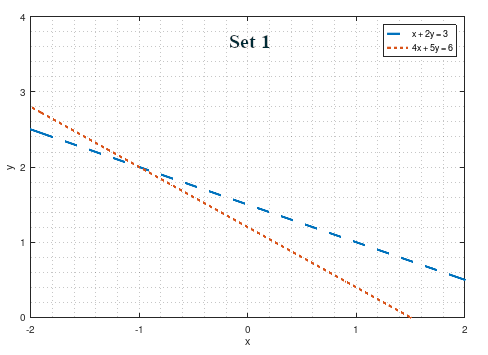
\includegraphics[height=10cm]{4a1}
		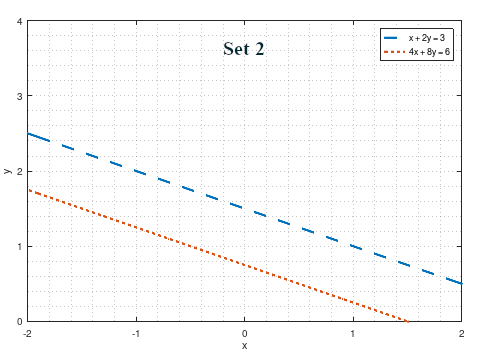
\includegraphics[height=10cm]{4a2}
	\end{figure}
\newpage
	\begin{figure}[h!]
		\centering
		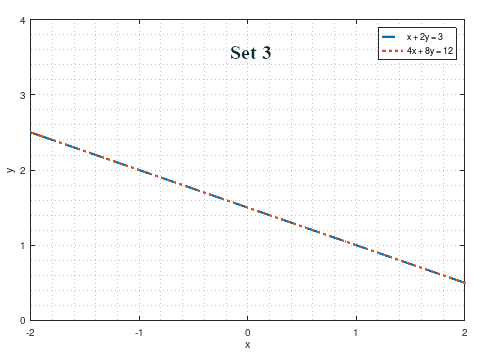
\includegraphics[height=10cm]{4a3}	
	\end{figure}
	Given system of linear equations for each set can be represented
	as straight lines on a 2D plane. Their intersection points corresponds to the possible solutions.\\
	Set 1: Unique solution at $(x,y) = (-1, 2)$\\
	Set 2: no solution (since both lines are parallel and not coincident)\\
	Set 3: infinite solutions (since both lines are parallel and coincident)\\

\newpage

\textbf{(4.b)} Each set of linear system of equations can be algebraically solved via elimination method or by using their matrix representation.\\
\\	
	\textbf{Set 1 (i) Elimination method:}
	\begin{equation*}
	\begin{split}
	&x + 2y = 3\\
	&\implies x = 3 -2y\\
	\\
	&4x + 5y = 6\\
	&\texttt{So,}~4(3- 2y) + 5y = 6\\
	&12 - 8y + 5y = 6\\
	&3y = 6 \\
	&y = 2\\
	\\
	&\implies x + 2\cdot 2 = 3\\
	&x = -1 
	\end{split}
	\end{equation*}
	\textbf{ (ii) Matrix method:}\\
	The system of equations can be written in matrix representation form as:
	\begin{equation*}
	\begin{split}
	\begin{pmatrix}
	1 &2\\
	4 &5
	\end{pmatrix}
	\begin{pmatrix}
	x\\
	y
	\end{pmatrix} =
	\begin{pmatrix}
	3\\
	6
	\end{pmatrix}
	\end{split}
	\end{equation*}
	which is of the form $\textbf{A}\cdot \textbf{x} = \textbf{b}$.
	\begin{equation*}
	\begin{split}
	\texttt{det}(\textbf{A}) &= ( 5 \cdot 1 - 2 \cdot 4 )\\
	&= -3
	\end{split}
	\end{equation*}
	det(\textbf{A}) is non zero. Hence the square matrix \textbf{A} is non-singular and $\textbf{A}^{-1}$ exists.\\
	Then $\textbf{x} = \textbf{A}^{-1}\textbf{b}$.
	
	\begin{equation*}
	\begin{split}
	\textbf{A}^{-1} &= \frac{1}{-3} \times 
	\begin{pmatrix}
	5 &-2\\
	-4 &1
	\end{pmatrix}\\
	\\
	&= \begin{pmatrix}
	-5/3 &2/3\\
	4/3 &-1/3
	\end{pmatrix}\\
	\end{split}
	\end{equation*}
	\begin{equation*}
	\begin{split}
	\textbf{x} &= \textbf{A}^{-1} \textbf{b}\\
	\\
	&= 
	\begin{pmatrix}
	-5/3 &2/3\\
	4/3 &-1/3	
	\end{pmatrix} \times 
	\begin{pmatrix}
	3\\
	6	
	\end{pmatrix}\\
	&= 
	\begin{pmatrix}
	-1\\
	2
	\end{pmatrix}
	\end{split}
	\end{equation*}
	$\therefore ~x = -1$ and $y = 2$ is the solution.
	
%%%%%%%%%%%%%%%%%%%%%%%%%%%%%%%%%%%%%%%%%%%%%
	\textbf{Set 2 (i) Elimination method:}
	\begin{equation*}
	\begin{split}
	&x + 2y = 3\\
	&\implies x = 3 -2y\\
	\\
	&4x + 8y = 6\\
	&\texttt{So,}~4(3- 2y) + 8y = 6\\
	&12 - 8y + 8y = 6\\
	&12 = 6 \\
	\end{split}
	\end{equation*}
	which is not true. Hence the system of equations has no solution.\\
	\\
	\textbf{ (ii) Matrix method:}\\
	The system of equations can be written in matrix representation form as:
	\begin{equation*}
	\begin{split}
	\begin{pmatrix}
	1 &2\\
	4 &8
	\end{pmatrix}
	\begin{pmatrix}
	x\\
	y
	\end{pmatrix} =
	\begin{pmatrix}
	3\\
	6
	\end{pmatrix}
	\end{split}
	\end{equation*}
	which is of the form $\textbf{A}\cdot \textbf{x} = \textbf{b}$.
	\begin{equation*}
	\begin{split}
	\texttt{det}(\textbf{A}) &= ( 8 \cdot 1 - 2 \cdot 4 )\\
	&= 0
	\end{split}
	\end{equation*}
	det(\textbf{A}) is zero. Hence the square matrix \textbf{A} is singular and $\textbf{A}^{-1}$ does not exist.\\
	Simplifying the system of equations,
	\begin{equation*}
	\begin{split}
	x + 2y &= 3\\
	x + 2y &= 3/2
	\end{split}
	\end{equation*}
	Subtracting first equation from the second equation, we get $0 = -3/2$. Since this is not possible for any combination of $x$ and $y$, this system of equations has no solutions.\\
%%%%%%%%%%%%%%%%%%%%%%%%%%%%%%%%%%%%%%%%%%%%%%%%%
	\textbf{Set 3 (i) Elimination method:}
	\begin{equation*}
	\begin{split}
	&x + 2y = 3\\
	&\implies x = 3 -2y\\
	\\
	&4x + 8y = 12\\
	&\texttt{So,}~4(3- 2y) + 8y = 12\\
	&12 - 8y + 8y = 12\\
	&12 = 12 \\
	\end{split}
	\end{equation*}
	which is true for infinitely many values of $x$ and $y$ which satisfies any one of the equations. Hence the system of equations has infinitely many solutions.\\
	\\
	\textbf{ (ii) Matrix method:}\\
	The system of equations can be written in matrix representation form as:
	\begin{equation*}
	\begin{split}
	\begin{pmatrix}
	1 &2\\
	4 &8
	\end{pmatrix}
	\begin{pmatrix}
	x\\
	y
	\end{pmatrix} =
	\begin{pmatrix}
	3\\
	12
	\end{pmatrix}
	\end{split}
	\end{equation*}
	which is of the form $\textbf{A}\cdot \textbf{x} = \textbf{b}$.
	\begin{equation*}
	\begin{split}
	\texttt{det}(\textbf{A}) &= ( 8 \cdot 1 - 2 \cdot 4 )\\
	&= 0
	\end{split}
	\end{equation*}
	det(\textbf{A}) is zero. Hence the square matrix \textbf{A} is singular and $\textbf{A}^{-1}$ does not exist.\\
	Simplifying the system of equations,
	\begin{equation*}
	\begin{split}
	x + 2y &= 3\\
	x + 2y &= 3
	\end{split}
	\end{equation*}
	Since both the equations in the system simplifies to the same equation, both lines have infinitely many coincident points and thus the system has infinitely many solutions.\\
%%%%%%%%%%%%%%%%%%%%%%%%%%%%%%%%%%%%%%%%%%%%%%%%%
\newpage

\textbf{(4.c)} For each set of linear system of equations, of the form:
\begin{equation*}
\begin{split}
a_1x + b_1y = c_1\\
a_2x + b_2y = c_2
\end{split}
\end{equation*}
\begin{equation*}
\begin{pmatrix}
a_1 &b_1\\
a_2 &b_2
\end{pmatrix}
\begin{pmatrix}
x\\
y
\end{pmatrix} = x
\begin{pmatrix}
a_1\\
a_2
\end{pmatrix}
+ y
\begin{pmatrix}
b_1\\
b_2
\end{pmatrix} =
\begin{pmatrix}
c_1\\
c_2
\end{pmatrix}
\end{equation*}
where,
\begin{equation*}
\begin{split}
\textbf{a} = 
\begin{pmatrix}
a_1\\
a_2
\end{pmatrix} \texttt{,}~
\textbf{b} = 
\begin{pmatrix}
b_1\\
b_2
\end{pmatrix}~ \texttt{and}~
\textbf{c} = 
\begin{pmatrix}
c_1\\
c_2
\end{pmatrix}
\end{split}
\end{equation*}
This can be thought of as checking whether the vector space spanned by the basis vectors $\textbf{a}$ and $\textbf{b}$ contains the vector $\textbf{c}$. If it does contain $\textbf{c}$, then that implies that atleast a solution exists for $x$ and $y$.\\
For the given sets, $a$ and $b$ may either span an $\mathbb{R}$ line or an $\mathbb{R}^{2}$ plane depending upon whether $a$ and $b$ are parallel or not.\\
\textbf{Set 1}\\
\begin{equation*}
\begin{pmatrix}
1 &2\\
4 &5\\
\end{pmatrix}
\begin{pmatrix}
x\\
y
\end{pmatrix} =
\begin{pmatrix}
3\\
6
\end{pmatrix}
\end{equation*}
Here,
\begin{equation*}
\begin{split}
a = \begin{pmatrix}
1\\
4
\end{pmatrix},~b = \begin{pmatrix}
2\\
5
\end{pmatrix}
\end{split}
\end{equation*}
Checking if $a$ and $b$ are parallel:\\
\begin{equation*}
\begin{split}
\theta &= cos^{-1} \left( \frac{a \cdot b}{|a||b|} \right)\\
&= cos^{-1} \left( \frac{2 + 20}{\sqrt{17} \cdot \sqrt{29}}\right)\\
&\neq 0
\end{split}
\end{equation*}
Since they are non-parallel, the vectors spans the entire $\mathbb{R}^{2}$ plane. So any vector $r \in \mathbb{R}^{2}$ like $c = (3~6)^{T}$ also lies on the $R^{2}$ plane and a unique solution exists.\\

\textbf{Set 2}\\
\begin{equation*}
\begin{pmatrix}
1 &2\\
4 &8\\
\end{pmatrix}
\begin{pmatrix}
x\\
y
\end{pmatrix} =
\begin{pmatrix}
3\\
6
\end{pmatrix}
\end{equation*}
Here,
\begin{equation*}
\begin{split}
a = \begin{pmatrix}
1\\
4
\end{pmatrix},~b = \begin{pmatrix}
2\\
8
\end{pmatrix}
\end{split}
\end{equation*}
But $b = 2\cdot a$, which means $b$ is a scaled version of the vector $a$. So $a$ and $b$ are parallel.\\
$c = (3~6)^{T}$ doesn't lie on the $\mathbb{R}$ line. Hence a solution $(x ~y)^{T}$ cannot be obtained in this case. Or in other words, no solutions exist.\\
\\
\textbf{Set 3}\\
\begin{equation*}
\begin{pmatrix}
1 &2\\
4 &8\\
\end{pmatrix}
\begin{pmatrix}
x\\
y
\end{pmatrix} =
\begin{pmatrix}
3\\
12
\end{pmatrix}
\end{equation*}

This is similar to \textbf{Set 2}, but the difference is that $c = (3~12)^{T} = 3 \cdot (1 ~ 4)^{T}$ lies on the specific $\mathbb{R}$ line. Which means that an infinte no of combinations of $x,y$ in $(x~y)^{T}$ is possible to arrive at $c$.  Hence the given set of linear equations has infinite number of solutions.
%%%%%%%%%%%%%%%%%%%%%%%%%%%%%%%%%%%%%%%%%%%%%%%%%

\newpage
\textbf{5.} 
\begin{align*}
\textbf{a} = 
\begin{pmatrix}
-209/362\\
-209/362\\
209/362
\end{pmatrix},~
\textbf{b} = 
\begin{pmatrix}
0\\
-408/577\\
-408/577
\end{pmatrix},~
\textbf{c} = 
\begin{pmatrix}
396/485\\
-198/485\\
198/485
\end{pmatrix}
\end{align*}
Rewriting,
\begin{equation*}
\begin{split}
\textbf{a} = 209/362 \times
\begin{pmatrix}
-1\\
-1\\
1
\end{pmatrix},~
\textbf{b} = 408/577 \times
\begin{pmatrix}
0\\
-1\\
-1
\end{pmatrix},~
\textbf{c} = 198/485 \times
\begin{pmatrix}
2\\
-1\\
1
\end{pmatrix}
\end{split}
\end{equation*}


\textbf{(5.a)} Dot product:
\begin{equation*}
\begin{split}
\textbf{a.b} &= \sum_{i=1}^{n} a_i b_i,~ \textbf{a,b} \in \mathbb{R}^n\\
 &= (209/362) \times (408/577) \times ((-1\cdot0) + (-1\cdot-1) + (1\cdot-1))\\
&= 0\\
\textbf{b.c} &= \sum_{i=1}^{n} b_i c_i,~ \textbf{b,c} \in \mathbb{R}^n\\
 &= (408/577) \times (198/485) \times ((0\cdot2) + (-1\cdot-1) + (-1\cdot1))\\
&= 0\\
\textbf{c.a} &= \sum_{i=1}^{n} c_i a_i,~ \textbf{c,a} \in \mathbb{R}^n\\
 &= (198/485) \times (209/362) \times ((2\cdot-1) + (-1\cdot-1) + (1\cdot1))\\
&= 0
\end{split}
\end{equation*}

\textbf{(5.b)} Geometric length:
\begin{equation*}
\begin{split}
\sqrt{\textbf{a.a}} &= \sqrt{\sum_{i=1}^{n} a_i a_i},~ \textbf{a} \in \mathbb{R}^n\\
 &= \sqrt{(209/362) \times (209/362) \times ((-1\cdot-1) + (-1\cdot-1) + (1\cdot1))}\\
&= 1\\
\sqrt{\textbf{b.b}} &= \sqrt{\sum_{i=1}^{n} b_i b_i},~ \textbf{b} \in \mathbb{R}^n\\
 &= \sqrt{(408/577) \times (408/577) \times ((0\cdot0) + (-1\cdot-1) + (-1\cdot-1))}\\
&= 1\\
\sqrt{\textbf{c.c}} &= \sqrt{\sum_{i=1}^{n} c_i c_i},~ \textbf{c} \in \mathbb{R}^n\\
 &= \sqrt{(198/485) \times (198/485) \times ((2\cdot2) + (-1\cdot-1) + (1\cdot1))}\\
&= 1\\
\\
\\
\textbf{x} &= \begin{pmatrix}
2\\
-40/57\\
8/77
\end{pmatrix}\\
\\
\sqrt{\textbf{x.x}} &= \sqrt{\sum_{i=1}^{n} x_i x_i},~ \textbf{x} \in \mathbb{R}^n\\
 &= \sqrt{(2\cdot2) + (-40/57 \cdot -40/57) + (8/77 \cdot 8/77)}\\
&\approx \sqrt{4 + 1600/3249 + 64/5929}\\
&\approx 2.12
\end{split}
\end{equation*}

\newpage
\textbf{(5.c)} 
\begin{equation*}
\begin{split}
\textbf{A} &= 
\begin{pmatrix}
-209/362 &0 &396/485\\
-209/362 &-408/577 &-198/485\\
209/362 &-408/577 &198/485
\end{pmatrix}\\
\\
\textbf{Ax} &= 
\begin{pmatrix}
-209/362 &0 &396/485\\
-209/362 &-408/577 &-198/485\\
209/362 &-408/577 &198/485
\end{pmatrix}
\times 
\begin{pmatrix}
2\\
-40/57\\
8/77
\end{pmatrix}\\
\\
&= \begin{pmatrix}
-1.070\\
-0.701\\
1.693
\end{pmatrix}\\
\\
\sqrt{\textbf{Ax}\cdot\textbf{Ax}} &= \sqrt{ (-1.070\cdot-1.070) + (-0.701\cdot-0.701) + (1.693\cdot1.693)}\\
&\approx \sqrt{1.145 + 0.491 + 2.866}\\
&\approx 2.12
\end{split}
\end{equation*}
It is observed that both $\sqrt{\textbf{Ax.Ax}}$ and $\sqrt{\textbf{x.x}}$ are equal.\\

\newpage
\textbf{(5.d)} 
\begin{equation*}
\begin{split}
\textbf{A}^{T}\textbf{A} &=
\begin{pmatrix}
-209/362 &-209/362 &209/362\\
0 &-408/577 &-408/577\\
396/485 &-198/485 &198/485
\end{pmatrix} \times
\begin{pmatrix}
-209/362 &0 &396/485\\
-209/362 &-408/577 &-198/485\\
209/362 &-408/577 &198/485
\end{pmatrix}\\
\\
&\approx \begin{pmatrix}
1 &0 &0\\
0 &1 &0\\
0 &0 &1
\end{pmatrix}\\
\\
\textbf{A}\textbf{A}^{T} &=
\begin{pmatrix}
-209/362 &0 &396/485\\
-209/362 &-408/577 &-198/485\\
209/362 &-408/577 &198/485
\end{pmatrix} \times
\begin{pmatrix}
-209/362 &-209/362 &209/362\\
0 &-408/577 &-408/577\\
396/485 &-198/485 &198/485
\end{pmatrix}\\
\\
&\approx \begin{pmatrix}
1 &0 &0\\
0 &1 &0\\
0 &0 &1
\end{pmatrix}
\end{split}
\end{equation*}
\\
\\
\textbf{(5.e)} To prove: If $\textbf{A}^{T}\textbf{A} = \textbf{A}\textbf{A}^{T} = \textbf{I}$, then $\sqrt{\textbf{Ax} \cdot \textbf{Ax}} = \sqrt{\textbf{x} \cdot \textbf{x}}$.
\begin{equation*}
\begin{split}
\textbf{Ax}\cdot \textbf{Ax} &= \left( \textbf{Ax} \right)^{T} \left( \textbf{Ax}\right)\\
&= \left(\textbf{x}^{T} \textbf{A}^{T}\right) \left( \textbf{A}\textbf{x}\right)\\
&= \textbf{x}^{T} \left( \textbf{A}^{T} \textbf{A} \right) \textbf{x}\\
&= \textbf{x}^{T} \textbf{I} \textbf{x}\\
&= \textbf{x}^{T} \textbf{x}\\
&= \textbf{x} \cdot \textbf{x}
\end{split}
\end{equation*}
which means\\
\\
$ \sqrt{\textbf{Ax}\cdot \textbf{Ax}} = \sqrt{\textbf{x} \cdot \textbf{x}}$\\
\newpage
\textbf{Why do you want to take this course and what are your expectations?}\\
\\
This course is relevant to my field of research. I expect to get a better grasp of how numerical linear algebra translates to practical applications.
\end{document}
